\documentclass[tikz,border=10pt]{standalone}
\usepackage{amsmath}
\usepackage{amssymb}
\usepackage{tikz}
\usetikzlibrary{arrows.meta,calc}

\definecolor{figazul}{RGB}{2,132,199}
\definecolor{figrojo}{RGB}{220,38,38}
\definecolor{figverde}{RGB}{22,163,74}

\begin{document}
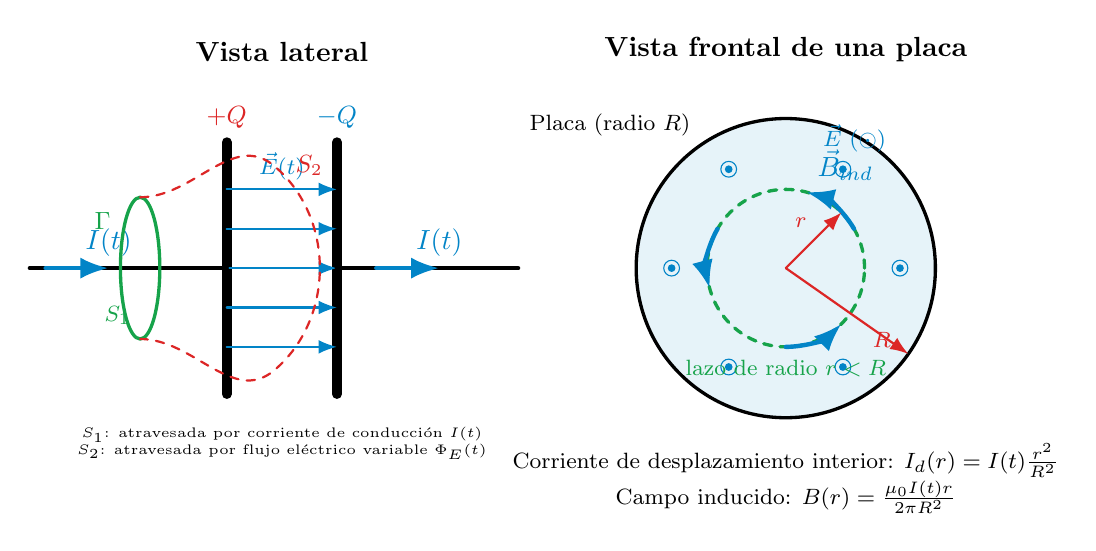
\begin{tikzpicture}[>=Latex, line cap=round, line join=round]
  % -------------------------------------------------------------
  % Panel Izquierdo: Vista lateral (Superficies S1 y S2)
  % -------------------------------------------------------------
  \begin{scope}[xshift=0cm]
    \node[above, font=\bfseries] at (0, 2.5) {Vista lateral};

    % Placas circulares paralelas vistas de canto
    % Placa izquierda (+Q) en x = -0.7
    \draw[line width=3.5pt] (-0.7, -1.6) -- (-0.7, 1.6);
    \node[above, font=\small\bfseries, color=figrojo] at (-0.7, 1.65) {$+Q$};

    % Placa derecha (-Q) en x = 0.7
    \draw[line width=3.5pt] (0.7, -1.6) -- (0.7, 1.6);
    \node[above, font=\small\bfseries, color=figazul] at (0.7, 1.65) {$-Q$};

    % Líneas de campo eléctrico uniforme E(t) entre las placas (de + a -)
    \foreach \y in {-1.0, -0.5, 0.0, 0.5, 1.0} {
      \draw[->, thick, color=figazul] (-0.7, \y) -- (0.7, \y);
    }
    \node[above, font=\footnotesize, color=figazul] at (0, 1.0) {$\vec{E}(t)$};

    % Cables rectos axiales
    % Cable de entrada (izquierda)
    \draw[ultra thick] (-3.2, 0) -- (-0.7, 0);
    \draw[->, ultra thick, color=figazul] (-3.0, 0) -- (-2.2, 0) node[above, color=figazul] {$I(t)$};

    % Cable de salida (derecha)
    \draw[ultra thick] (0.7, 0) -- (3.0, 0);
    \draw[->, ultra thick, color=figazul] (1.2, 0) -- (2.0, 0) node[above, color=figazul] {$I(t)$};

    % Lazo amperiano Gamma alrededor del cable en x = -1.8
    \draw[very thick, color=figverde] (-1.8, 0) ellipse (0.25 and 0.9);
    \node[left, font=\small\bfseries, color=figverde] at (-2.05, 0.6) {$\Gamma$};

    % Superficie S1: disco plano que tapa Gamma (atravesada por el cable)
    \node[left, font=\footnotesize, color=figverde] at (-1.8, -0.6) {$S_1$};

    % Superficie S2: forma de bolsa que pasa entre las placas sin tocar el cable
    \draw[thick, dashed, color=figrojo]
      (-1.8, 0.9) to[out=0, in=140] (-0.1, 1.3)
      to[out=-40, in=40] (-0.1, -1.3)
      to[out=220, in=0] (-1.8, -0.9);
    \node[right, font=\small\bfseries, color=figrojo] at (0.05, 1.3) {$S_2$};

    % Cota de separación d o nota
    \node[below, font=\tiny, align=center] at (0, -1.9) {
      $S_1$: atravesada por corriente de conducci\'on $I(t)$ \\
      $S_2$: atravesada por flujo el\'ectrico variable $\Phi_E(t)$
    };
  \end{scope}

  % -------------------------------------------------------------
  % Panel Derecho: Vista frontal de una placa
  % -------------------------------------------------------------
  \begin{scope}[xshift=6.4cm]
    \node[above, font=\bfseries] at (0, 2.5) {Vista frontal de una placa};

    % Placa circular de radio R = 1.9
    \draw[very thick, fill=figazul!10] (0, 0) circle (1.9);
    \node[above left, font=\footnotesize] at (125:1.9) {Placa (radio $R$)};

    % Campo eléctrico E saliente (\odot) entre las placas
    \foreach \ang in {0, 60, 120, 180, 240, 300} {
      \draw[thin, color=figazul] (\ang:1.45) circle (0.10);
      \fill[color=figazul] (\ang:1.45) circle (1.4pt);
    }
    \node[above right, font=\footnotesize, color=figazul] at (0.35, 1.35) {$\vec{E}$ ($\odot$)};

    % Lazo circular coaxial de radio r < R (en verde)
    \draw[very thick, dashed, color=figverde] (0, 0) circle (1.0);
    \node[below, font=\footnotesize, color=figverde] at (0, -1.05) {lazo de radio $r < R$};

    % Campo magnético B_ind inducido azimutal a lo largo del lazo
    \draw[->, ultra thick, color=figazul] (30:1.0) arc (30:75:1.0) node[above right, color=figazul] {$\vec{B}_{ind}$};
    \draw[->, ultra thick, color=figazul] (150:1.0) arc (150:195:1.0);
    \draw[->, ultra thick, color=figazul] (270:1.0) arc (270:315:1.0);

    % Cota del radio r (en rojo)
    \draw[->, thick, color=figrojo] (0, 0) -- (45:1.0);
    \node[above left, color=figrojo, font=\footnotesize] at (45:0.55) {$r$};

    % Cota del radio exterior R de la placa (en rojo)
    \draw[->, thick, color=figrojo] (0, 0) -- (-35:1.9);
    \node[below right, color=figrojo, font=\footnotesize] at (-35:1.2) {$R$};

    % Resultado de Ampère-Maxwell
    \node[below, font=\footnotesize, align=center] at (0, -2.1) {
      Corriente de desplazamiento interior: $I_d(r) = I(t)\frac{r^2}{R^2}$ \\
      Campo inducido: $B(r) = \frac{\mu_0 I(t) r}{2\pi R^2}$
    };
  \end{scope}
\end{tikzpicture}
\end{document}
